\section{La reproduction des battraciens}



\section{La différenciation mâle/femelle}

Si le sexe est déterminé génétiquement, il est modulé par les conditions thermiques. Si l’hiver a été doux et bref, la production d’individus hermaphrodites augmente dans la population.
La différenciation sexuelle est postérieure à la métamorphose et a lieu lors de la croissance.
Le mâle possède une taille légèrement plus petite que la femelle.
La maturité sexuelle est acquise plus ou moins tardivement (en 3 ans pour la grenouille rousse). A partir de ce stade, en théorie, la croissance se poursuit lentement et indéfiniment. La grenouille vit en moyenne 5 ans, sa longévité maximale est de 15 ans.
        
\section{Le choix du partenaire}
En mars, les grenouilles sortent de leur hibernation.  Dès que la température extérieure atteint environ 7deg C, les individus se mettent en route vers le site de reproduction, s’il n’était pas déjà sur place. Chez la plupart des espèces, l’accouplement a lieu dans l’eau.

Les femelles, encore à quelques kilomètres de distance, perçoivent le cri nuptial émis par leurs congénères grâce aux gonflements des sacs vocaux.


\begin{figure}%
	\begin{center}
	\includegraphics[width=0.7\textwidth]{laRepro/sacvoval.jpg}	
	\end{center}
	\caption{Gonflement des sacs vocaux permettant l'émission de son.}%
	\label{fig:encordee}%
\end{figure}


 
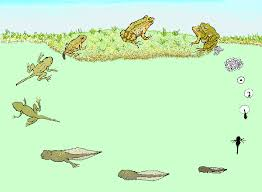
\includegraphics[width=0.7\textwidth]{laRepro/cycleReproduction.jpg}